\chapter{Анализ эффективности программного комплекса NonLocFEM}\label{ch:NonLocFEMAnalysis} 

\section{Тестирование алгоритма ассемблирования матриц}\label{sec:NumericalMethods/AssemblyTest}

Оценим масштабируемость полученного алгоритма ассемблирования матриц теплопроводности и жёсткости (\ref{eq:ApproxNonlocParallel}). Для этого проведём серию расчётов на вычислительном кластере, в состав которого входит 6 вычислительных узлов. На каждом узле кластера установлен 18-ядерный процессор Intel Core i9 10980XE и 128 ГБ оперативной памяти DDR4. Будем рассматривать тестовые задачи на прямоугольной области $S = \{ \boldsymbol{x} | -5 \leqslant x_1 \leqslant 5, -0.5 \leqslant x_2 \leqslant 0.5 \}$, с введённой на ней равномерной сеткой $S_h$. Как и в предыдущей главе, все вычисления проведены с использованием квадратичных серендиповых элементов, интегрирование выполнено гауссовыми квадратурами 3-го порядка (9 квадратурных узлов), а в качестве функции нелокального влияния выбрана $\varphi = \varphi_{2,1}^P$, выбор которой также обоснован в предыдущей главе. Хранение разреженных матриц организовано в формате CSR \cite{Pisanetzkiy}, где для хранения индексов использовались 64-битные целые числа, а для хранения коэффициентов числа с плавающей точкой двойной точности. Также была учтена симметрия матрицы, то есть для хранения и вычисления использовалась только верхняя половина \mbox{матрицы.}

Начнём исследование масштабируемости алгоритмов на машинах с общей памятью, то есть задействуем только один узел кластера и технологию параллельного программирования OpenMP. Для этого проведём серию расчётов варьируя разбиение сетки $h$ и радиус нелокальности $r$, который в данном исследовании совпадает с радиусом поиска. Результаты, представленные в Таблице~\ref{tab:OpenMP}, свидетельствуют о том, что для хранения матрицы жёсткости $\widehat{\textbf{K}}_E$ требуется в 4 раза больше оперативной памяти, чем для матрицы теплопроводности $\widehat{\textbf{K}}_T$ на аналогичной сетке, что было ожидаемо, учитывая размерности блоков матриц теплопроводности (\ref{eq:ThermalBlock}) и жёсткости (\ref{eq:StressBlock}). В обоих случаях, темпы роста занимаемой оперативной памяти относительно разбиения сетки линейные в классическом случае и квадратичные в нелокальном. При сравнении времён сборки матриц можем отметить, что в классическом случае время ассемблирования матрицы жёсткости $\widehat{\textbf{K}}_E$ приблизительно в 3 раза дольше, чем матрицы теплопроводности $\widehat{\textbf{K}}_T$, однако, в нелокальном случае эта разница сокращается до 1.2, чего удалось достичь за счёт оптимизации вычислений с использованием блочного подхода в ассемблировании.

\begin{table}[htbp]
    \centering
    \begin{threeparttable}% выравнивание подписи по границам таблицы
        \caption{Требуемая оперативная память и затрачиваемое время при ассемблировании матриц теплопроводности и жёсткости с использованием технологии OpenMP}\label{tab:OpenMP}
        \begin{tabular}{|c|c|c|c|c|c|c|c|}
	\hline
	Количество & Радиус & \multicolumn{2}{c|}{Требуемая}   & \multicolumn{2}{c|}{Время, с} & \multicolumn{2}{c|}{Время, с} \\
	элементов  & поиска & \multicolumn{2}{c|}{оперативная память} & \multicolumn{2}{c|}{1 поток}  & \multicolumn{2}{c|}{18 потоков} \\
	\cline{3-8}
	      &        & $\widehat{\textbf{K}}_T$ & $\widehat{\textbf{K}}_E$ & $\widehat{\textbf{K}}_T$ & $\widehat{\textbf{K}}_E$ & $\widehat{\textbf{K}}_T$ & $\widehat{\textbf{K}}_E$ \\
	\hline
	$400 \times 40$   & 0    & 6.2 Мб  & 23.8 Мб & 0.061 & 0.187 & 0.028 & 0.048 \\
	\hline
	$800 \times 80$   & 0    & 24.5 Мб & 95 Мб   & 0.521 & 1.701 & 0.116 & 0.274 \\
	\hline
	$1600 \times 160$ & 0    & 97.8 Мб & 379 Мб  & 5.17  & 16.76 & 0.705 & 2.366 \\
	\hline
	$400 \times 40$   & 0.05 & 61.4 Мб & 244 Мб  & 14.4  & 17.06 & 1.055 & 1.288 \\
	\hline
	$800 \times 80$   & 0.05 & 548 Мб  & 2.2 Гб  & 157   & 187   & 11.37 & 13.3  \\
	\hline
	$1600 \times 160$ & 0.05 & 5.5 Гб  & 22 Гб   & 1825  & 2166  & 132.9 & 155   \\
	\hline
	$400 \times 40$   & 0.1  & 133 Мб  & 532 Мб  & 38    & 44.9  & 2.68  & 3.26  \\
	\hline
	$800 \times 80$   & 0.1  & 1.34 Мб & 5.4 Гб  & 450   & 529   & 32    & 37.8  \\
	\hline
	$1600 \times 160$ & 0.1  & 17 Гб   & 68 Гб   & 6134  & 7266  & 447   & 521   \\
	\hline
        \end{tabular}
    \end{threeparttable}
\end{table}

Обращаясь к результатам из Таблицы \ref{tab:OpenMP}, можем построить диаграммы эффективности распараллеливания алгоритмов ассемблирования матриц теплопроводности и жёсткости. Исходя из полученных результатов, представленных на Рис. \ref{fig:OMPParallelization}, отметим достаточно хорошую эффективность распараллеливания, которая в нелокальном случае достигает 14 раз при использовании всех 18 ядер процессора. Однако ускорение в классическом случае не такое высокое, что можно объяснить обобщённостью используемых алгоритмов формирования портрета матрицы, которые недостаточно эффективно работают на малых объёмах данных.

\begin{figure}[ht]
    \begin{minipage}[b][][b]{0.49\linewidth}\centering
        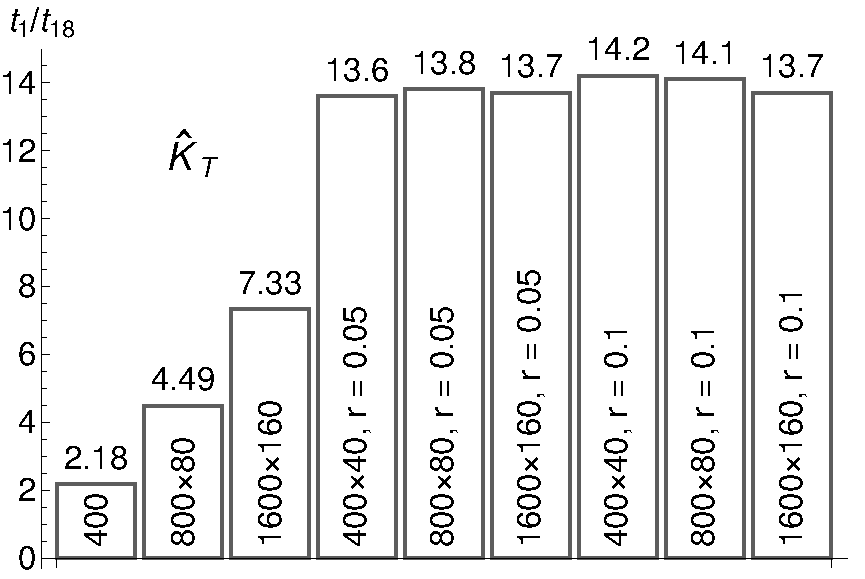
\includegraphics[width=\linewidth]{pics/OMPThermal.pdf} \\ а)
    \end{minipage}
    \hfill
    \begin{minipage}[b][][b]{0.49\linewidth}\centering
        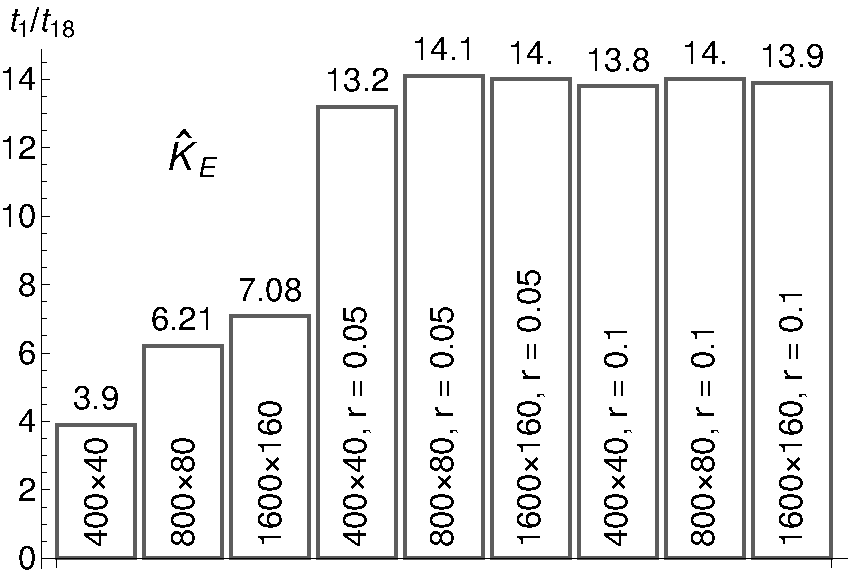
\includegraphics[width=\linewidth]{pics/OMPMechanical.pdf} \\ б)
    \end{minipage}
    \caption{Эффективность распараллеливания алгоритма сборки матриц (а)~теплопроводности и (б)~жёсткости при использовании технологии OpenMP}
    \label{fig:OMPParallelization}
\end{figure}

Теперь исследуем масштабируемость алгоритма ассемблирования матриц на примере использования технологии MPI. Здесь сконцентрируем внимание на алгоритме балансировки данных между процессами, так как вопрос хранения матриц в классе нелокальных задач стоит наиболее остро. Для этого будем рассматривать ту же область, но возьмём более подробную сетку $S_h$, состояющую из $3200 \times 320$ элементов. Радиус нелокальности $r$ выберем равным 0.1. С целью исключения дублирования результатов, остановимся на рассмотрении лишь матрицы теплопроводности.

Проведём сравнение двух запусков на 6 вычислительных узлах кластера. Первый запуск осуществим без балансировки данных, то есть распределения узлов сетки между процессами оставим равномерным. Второй запуск осуществим с балансировкой данных между процессами, которая выполняется по алгоритму описанному в третьей главе. На Рис. \ref{fig:MPIBalance} представлены полученные распределения затрачиваемой оперативной памяти для хранения блоков матрицы на каждом узле. В варианте без балансировки данные распределены не равномерно и некоторым узлам кластера достался объём данных больше, чем другим. В варианте с балансировкой данные распределены, в рамках допустимой погрешности, равномерно. Из чего можно сделать вывод, что алгоритм балансировки данных работает корректно.

\begin{figure}[ht]
    \begin{minipage}[b][][b]{0.49\linewidth}\centering
        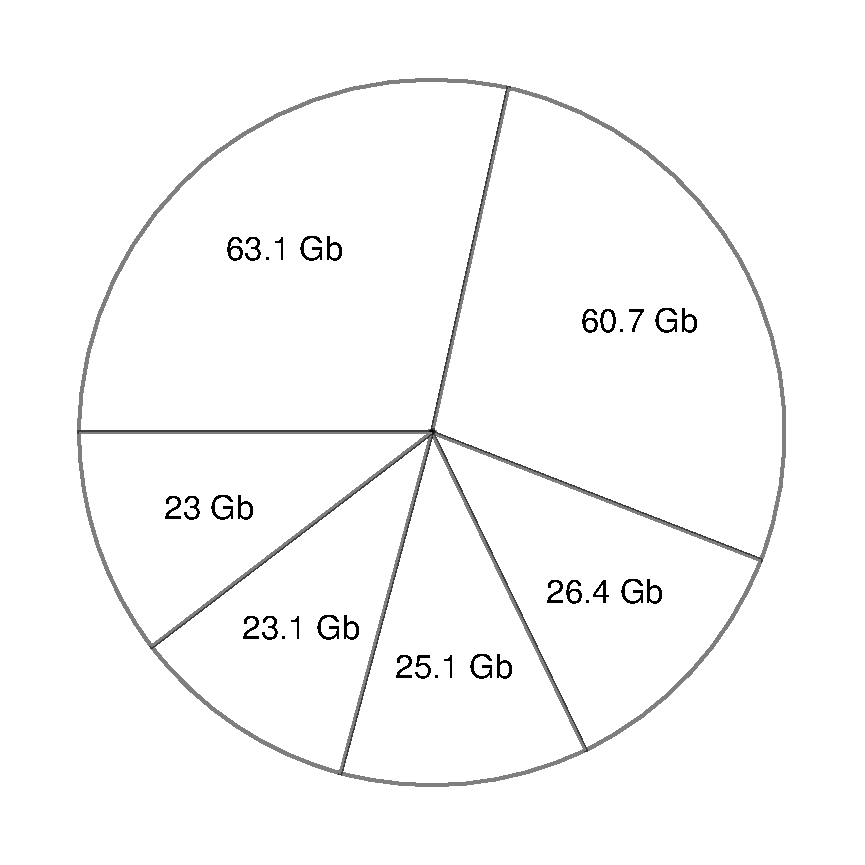
\includegraphics[width=\linewidth]{pics/PieChartNoBalance.pdf} \\ а)
    \end{minipage}
    \hfill
    \begin{minipage}[b][][b]{0.49\linewidth}\centering
        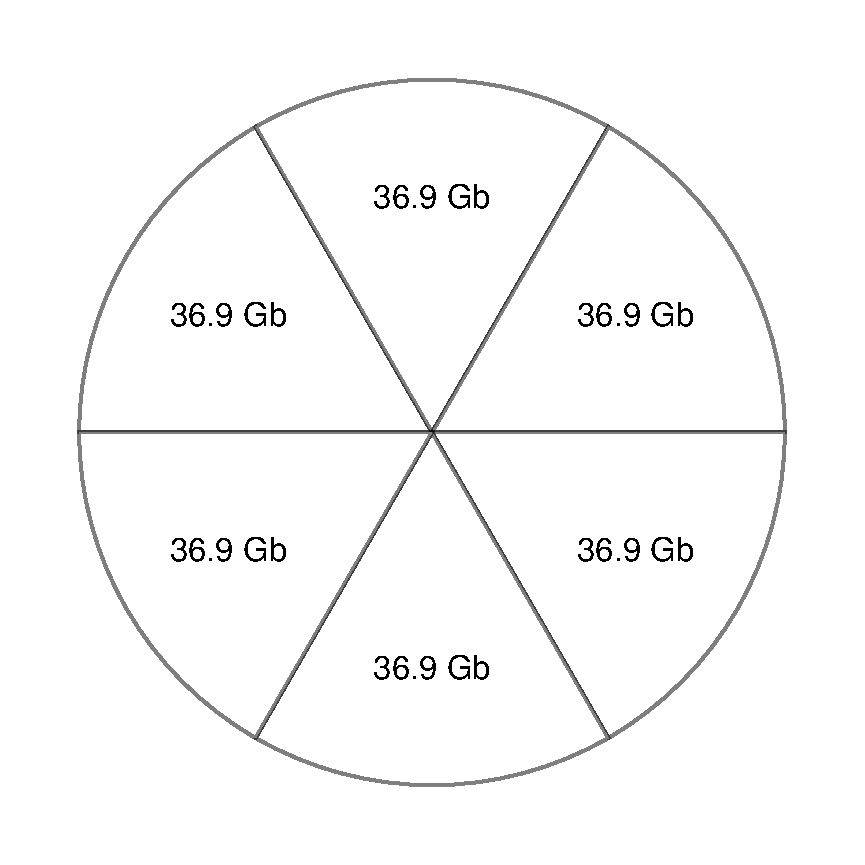
\includegraphics[width=\linewidth]{pics/PieChartBalance.pdf} \\ б)
    \end{minipage}
    \caption{Распределение размеров блоков матрицы теплопроводности между 6 процессами в случае (а) без балансировки и (б) с балансировкой данных}
    \label{fig:MPIBalance}
\end{figure}

В качестве замечания можно ещё отметить, что алгоритм балансировки данных также ускоряет работу метода сопряжённых градиентов, так как операция умножения матрицы на вектор становится одинаковой по трудозатратам на каждом узле кластера. Более подробно про другие возможные методы ускорения сходимости решателей СЛАУ обсудим в последующих разделах.

\section{Анализ скорости сходимости при оптимизации базиса конечных элементов}\label{sec:NumericalMethods/BasisOptimization}

В работе повсеместно использовались квадратичные серендиповые элементы, в связи с чем возникла потребность оптимизиации их базиса для ускорения сходимости итерационных методов решения СЛАУ. Отметим, что у квадратичного серендипового элемента есть целое параметрическое семейство базисов, представленное в третьей главе диссертации. В той же главе была получена оценка оптимального значения параметра $s$ (\ref{eq:ParamSOptimal}) согласно которой скорость сходимости должна быть максимальной в точке $s = 2/9$. Проверим эту оценку на практике, а заодно исследуем влияние других параметров модели.

Для проверки корректности оценки решим серию задач варьируя параметр $s$. Расчёты снова будем проводить на прямоугольной области $S = \{ \boldsymbol{x} \ | \ -5 \leqslant x_1 \leqslant 5, -0.5 \leqslant x_2 \leqslant 0.5  \}$, с введённой на этой области равномерной сеткой $S_h = 1000 \times 100$. Обезразмерим уравнения (\ref{eq:StationaryHeatEquation}) и (\ref{eq:EquilibriumEquation}) относительно коэффициента теплопроводности $\lambda$ и модуля Юнга $E$ соответственно
\begin{gather*}
	\overline{\boldsymbol{q}} = \dfrac{\boldsymbol{q}}{\lambda},
	\quad
	\overline{\boldsymbol{\sigma}} = \dfrac{\widehat{\boldsymbol{\sigma}}}{E},
\end{gather*}
так как параметры $\lambda$ и $E$ в данном случае выступают в роли масштабирующих множителей для собственных чисел матриц $\widehat{\textbf{K}}_T$ и $\widehat{\textbf{K}}_E$ соответственно. Коэффициент Пуассона $\nu$ примем равным 0.3. Поставим граничные условия для уравнения теплопроводности
\begin{gather*}
	\boldsymbol{n} \cdot \overline{\boldsymbol{q}} |_{x_1 = -5} = -1,
	\quad
	\boldsymbol{n} \cdot \overline{\boldsymbol{q}} |_{x_1 = 5} = 1,
	\quad
	\int\limits_S T dS = 0,
\end{gather*}
и для уравнения равновесия
\begin{gather*}
	n_j \overline{\sigma}_{j1} |_{x_1 = -5} = -1,
	\quad
	n_j \overline{\sigma}_{j1} |_{x_1 = 5} = 1,
	\quad
	u_1 |_{x_1 = 0} = 0,
	\quad
	u_2 |_{x_2 = 0} = 0.
\end{gather*}
Решение СЛАУ будем искать методом сопряжённых градиентов без использования каких-либо дополнительных предобуславливателей.

Для определения числа обусловленности (\ref{eq:CondValue}) необходимо вычислить максильное и минимальное собственные числа матрицы. Для их вычисления к программному комплексу NonLocFEM была подключена библиотека Spectra \cite{SpectraLib}, которая позволяет вычислять собственные числа разреженных матриц и совместима с библиотекой линейной алгебры Eigen \cite{EigenLib}.

В ходе экспериментов было установлено, что минимальное собственное число $\lambda_{\min}$ не зависит от параметра базиса $s$ и вариаций функции нелокальности $\varphi$, но при этом имеет некоторую зависимость от вклада нелокального влияния и радиуса нелокальности $r$, где при их увеличении величина собственного числа $\lambda_{\min}$ начинает уменьшаться. Однако исходя из результатов, представленных в Таблицах \ref{tab:ThermalEigenMin} и \ref{tab:StressEigenMin}, можем сделать вывод, что зависимость от параметров модели весьма слабая, так как величина изменений не достигает и десятой доли от числа полученного в классическом случае, то есть минимальное собственное число не оказывает серьёзного влияния на число обусловленности. Также можно отметить, что минимальные собственные числа матриц теплопроводности и жёсткости при одинаковых параметрах модели достаточно близки по значениям.

\begin{table}[htbp]
    \centering
    \begin{threeparttable}% выравнивание подписи по границам таблицы
        \caption{Зависимость минимального собственного числа матрицы теплопроводности $\widehat{\textbf{K}}_T$ от параметров модели $p_1$ и $r$}\label{tab:ThermalEigenMin}
        \begin{tabular}{|c|c|c|c|c|}
			\hline
			\backslashbox{$r$}{$p_1$} & 1 & 0.75 & 0.5 & 0.25 \\
			\hline
			0    & $3.2637 \cdot 10^{-6}$ & --- & --- & --- \\
			\hline
			0.05 & --- & $3.2429 \cdot 10^{-6}$ & $3.2181 \cdot 10^{-6}$ & $3.1793 \cdot 10^{-6}$ \\
			\hline
			0.1  & --- & $3.2231 \cdot 10^{-6}$ & $3.1750 \cdot 10^{-6}$ & $3.0997 \cdot 10^{-6}$ \\
			\hline
			0.15 & --- & $3.2032 \cdot 10^{-6}$ & $3.1319 \cdot 10^{-6}$ & $3.0218 \cdot 10^{-6}$ \\
			\hline
        \end{tabular}
    \end{threeparttable}
\end{table}

\begin{table}[htbp]
    \centering
    \begin{threeparttable}% выравнивание подписи по границам таблицы
        \caption{Зависимость минимального собственного числа матрицы жёсткости $\widehat{\textbf{K}}_E$ от параметров модели $p_1$ и $r$}\label{tab:StressEigenMin}
        \begin{tabular}{|c|c|c|c|c|}
			\hline
			\backslashbox{$r$}{$p_1$} & 1 & 0.75 & 0.5 & 0.25 \\
			\hline
			0    & $3.2614 \cdot 10^{-6}$ & --- & --- & --- \\
			\hline
			0.05 & --- & $3.2471 \cdot 10^{-6}$ & $3.2328 \cdot 10^{-6}$ & $3.1958 \cdot 10^{-6}$ \\
			\hline
			0.1  & --- & $3.2336 \cdot 10^{-6}$ & $3.1911 \cdot 10^{-6}$ & $3.1191 \cdot 10^{-6}$ \\
			\hline
			0.15 & --- & $3.2183 \cdot 10^{-6}$ & $3.1489 \cdot 10^{-6}$ & $3.0435 \cdot 10^{-6}$ \\
			\hline
        \end{tabular}
    \end{threeparttable}
\end{table}

Максимальные собственные числа $\lambda_{\max}$ матриц теплопроводности $\widehat{\textbf{K}}_T$ и жёсткости $\widehat{\textbf{K}}_E$ напротив имеют достаточно сильную зависимость как от параметра базиса $s$, так и от весового параметра модели $p_1$. При этом зависимость от весового параметра $p_1$ удаётся установить эмпирически, она в точности равна $\lambda_{\max}^{NL}(s) = p_1 \lambda_{\max}^{L}(s)$. Зависимость от радиуса нелокальности $r$ и функции нелокальности $\varphi$ у максимальных собственных чисел отсутствует. Результаты представлены в Таблицах \ref{tab:ThermalIterAndMaxEgien} и \ref{tab:MechanicalIterAndMaxEgien}, где также представлены данные о количествах итераций метода сопряжённых градиентов.

\begin{table}[htbp]
    \centering
    \begin{threeparttable}% выравнивание подписи по границам таблицы
        \caption{Зависимости количества итераций $N$ и максимального собственного числа $\lambda_{\max}$ матрицы теплопроводности $\widehat{\textbf{K}}_T$ от вариации параметров $p_1$ и $s$}\label{tab:ThermalIterAndMaxEgien}
        \begin{tabular}{|c|c|c|c|c|c|c|c|c|}
			\hline
			Значение & \multicolumn{2}{c|}{$p_1 = 1$} & \multicolumn{2}{c|}{$p_1 = 0.75$} & \multicolumn{2}{c|}{$p_1 = 0.5$} & \multicolumn{2}{c|}{$p_1 = 0.25$} \\ 
			\cline{2-9}
			параметра $s$ & $N$  & $\lambda_{\max}$ & $N$  & $\lambda_{\max}$ & $N$  & $\lambda_{\max}$ & $N$  & $\lambda_{\max}$ \\ 
			\hline
			-1/3 & 6961 & 15.997 & 8724 & 11.997 & 5036 & 7.9980 & 3549 & 3.9984 \\
			\hline
			-2/9 & 5600 & 11.198 & 5110 & 8.3986 & 4341 & 5.5987 & 2948 & 2.7990 \\
			\hline
			-1/9 & 4540 & 7.4660 & 4095 & 5.5993 & 3367 & 3.7327 & 2360 & 1.8663 \\
			\hline
			   0 & 3868 & 5.3332 & 3640 & 3.9997 & 2891 & 2.6662 & 1961 & 1.3328 \\
			\hline
			 1/9 & 3885 & 5.3332 & 3442 & 3.9997 & 2861 & 2.6662 & 1947 & 1.3328 \\
			\hline 
			 2/9 & 4000 & 5.3332 & 3600 & 3.9997 & 2826 & 2.6662 & 2003 & 1.3328 \\
			\hline 
			 1/3 & 3889 & 5.3332 & 3567 & 3.9997 & 2778 & 2.6662 & 1948 & 1.3328 \\
			\hline 
			 4/9 & 3786 & 5.3332 & 3474 & 3.9997 & 2835 & 2.6662 & 1982 & 1.3328 \\
			\hline 
			 5/9 & 4719 & 7.4660 & 4415 & 5.5993 & 3525 & 3.7327 & 2353 & 1.8663 \\
			\hline 
			 2/3 & 5761 & 11.198 & 6887 & 8.3986 & 4134 & 5.5987 & 2982 & 2.7990 \\
			\hline 
			 7/9 & 7218 & 15.997 & 6349 & 11.997 & 5285 & 7.9980 & 3720 & 3.9984 \\
			\hline
        \end{tabular}
    \end{threeparttable}
\end{table}

\begin{table}[htbp]
    \centering
    \begin{threeparttable}% выравнивание подписи по границам таблицы
        \caption{Зависимости количества итераций $N$ и максимального собственного числа $\lambda_{\max}$ матрицы жёсткости $\widehat{\textbf{K}}_E$ от вариации параметров $p_1$ и $s$}\label{tab:MechanicalIterAndMaxEgien}
        \begin{tabular}{|c|c|c|c|c|c|c|c|c|}
			\hline
			Значение & \multicolumn{2}{c|}{$p_1 = 1$} & \multicolumn{2}{c|}{$p_1 = 0.75$} & \multicolumn{2}{c|}{$p_1 = 0.5$} & \multicolumn{2}{c|}{$p_1 = 0.25$} \\ 
			\cline{2-9}
			параметра $s$ & $N$  & $\lambda_{\max}$ & $N$  & $\lambda_{\max}$ & $N$  & $\lambda_{\max}$ & $N$  & $\lambda_{\max}$ \\ 
			\hline
			-1/3 & 7454 & 13.061 & 6549 & 9.7954 & 4758 & 6.5298 & 3893 & 3.2650 \\
			\hline
			-2/9 & 6261 & 9.6366 & 5066 & 7.2272 & 4402 & 4.8178 & 3344 & 2.4090 \\
			\hline
			-1/9 & 4805 & 7.0840 & 4820 & 5.3128 & 3992 & 3.5416 & 2870 & 1.7707 \\
			\hline
			   0 & 4797 & 5.4194 & 3996 & 4.0643 & 3053 & 2.7094 & 2509 & 1.3545 \\
			\hline   
			 1/9 & 4380 & 4.5195 & 3320 & 3.3897 & 2703 & 2.2602 & 2289 & 1.1306 \\
			\hline 
			 2/9 & 4272 & 4.2968 & 3296 & 3.2222 & 2727 & 2.1476 & 2229 & 1.0730 \\
			\hline 
			 1/3 & 4270 & 4.2970 & 3551 & 3.2224 & 2641 & 2.1477 & 2229 & 1.0731 \\
			\hline 
			 4/9 & 4085 & 4.3423 & 3772 & 3.2566 & 3124 & 2.1709 & 2242 & 1.0852 \\
			\hline 
			 5/9 & 4446 & 6.1015 & 3911 & 4.5760 & 3704 & 3.0504 & 2659 & 1.5249 \\
			\hline 
			 2/3 & 6138 & 8.8614 & 4814 & 6.6458 & 4464 & 4.4302 & 3203 & 2.2147 \\
			\hline 
			 7/9 & 7076 & 12.436 & 5567 & 9.3273 & 4634 & 6.2178 & 3802 & 3.1083 \\
			\hline
        \end{tabular}
    \end{threeparttable}
\end{table}

Теперь рассмотрим данные из таблиц \ref{tab:ThermalEigenMin}-\ref{tab:MechanicalIterAndMaxEgien} в графическом представлении. На Рис. \ref{fig:ThermalCondAndIter} представлены зависимости числа обсусловленности и количества итераций метода сопряжённых градиентов от параметра базиса $s$ и весового параметра модели $p_1$. Обратим внимание, что кривые числа обусловленности симметричные относительно точки $s = 2/9$, а также, что число обусловленности снижается по мере уменьшения весового параметра $p_1$. Также стоит отметить, что на интервале $0 \leqslant s \leqslant 4/9$ кривые числа обусловленности выходят на плато, центром которого по прежнему является точка $s = 2/9$. Кривые зависимости числа итераций хорошо коррелируют с кривыми числа обусловленности и минимум числа итераций находится в окрестностях точки $s = 2/9$, а увеличение вклада нелокального влияния ускоряет сходимость метода при заданных параметрах.



Результаты, представленные на Рис. \ref{fig:MechanicalCondAndIter}, для матрицы жёсткости аналогичны результатам, представленным на Рис. \ref{fig:ThermalCondAndIter}, для матрицы теплопроводности, однако, здесь графики зависимости числа обусловленности от параметра $s$ уже не являются симметричными и плато на них уже менее выражено, а графики зависимости числа итераций хуже коррелируют с графиками числа обусловленности. Тем ни менее, минимум числа обусловленности и числа итераций по прежнему находится в окрестностях точки $s = 2/9$ из чего можно сделать вывод, что оценка (\ref{eq:ParamSOptimal}) пригодна для практического использования.

Также важно отметить, что несмотря на то, что количество итераций в нелокальном случае становится меньше, время затрачиваемое на решение СЛАУ в нелокальном случае может быть на несколько порядков больше, чем для аналогичной задачи в классическом случае. Это связано с объёмами данных, которые занимают матрицы в нелокальном случае и главным сдерживающим фактором в скорости решения СЛАУ выступает скорость работы оперативной памяти, а не процессора.

\begin{figure}[ht]
    \begin{minipage}[b][][b]{0.49\linewidth}\centering
        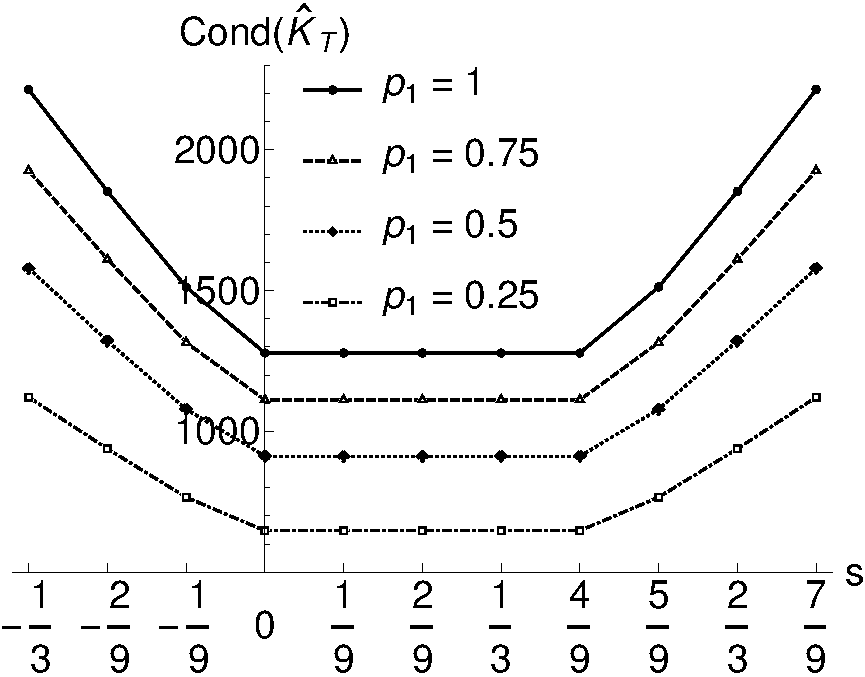
\includegraphics[width=\linewidth]{pics/ThermalCond.pdf} \\ а)
    \end{minipage}
    \hfill
    \begin{minipage}[b][][b]{0.49\linewidth}\centering
        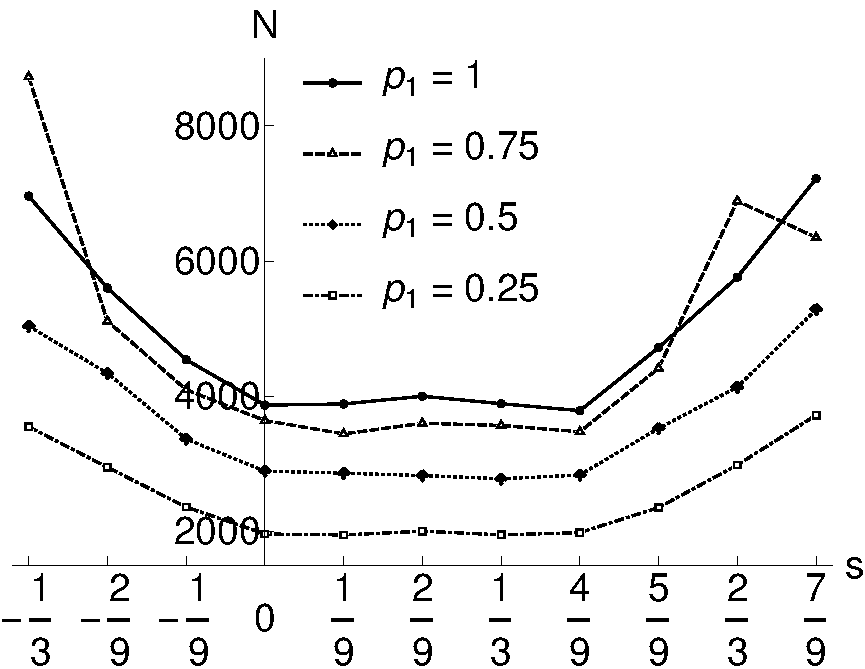
\includegraphics[width=\linewidth]{pics/ThermalIter.pdf} \\ б)
    \end{minipage}
    \caption{Зависимость (а) числа обусловленности и (б) количества итераций $N$ для матрицы теплопроводности $\widehat{\textbf{K}}_T$ от параметров $s$ и $p_1$ при $r = 0.1$}
    \label{fig:ThermalCondAndIter}
\end{figure}

\begin{figure}[ht]
    \begin{minipage}[b][][b]{0.49\linewidth}\centering
        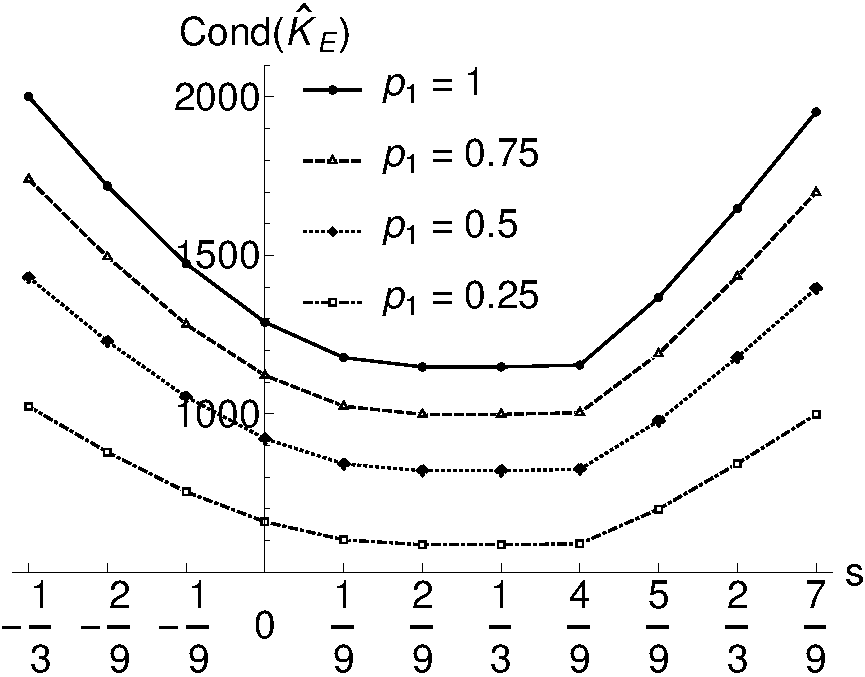
\includegraphics[width=\linewidth]{pics/MechanicalCond.pdf} \\ а)
    \end{minipage}
    \hfill
    \begin{minipage}[b][][b]{0.49\linewidth}\centering
        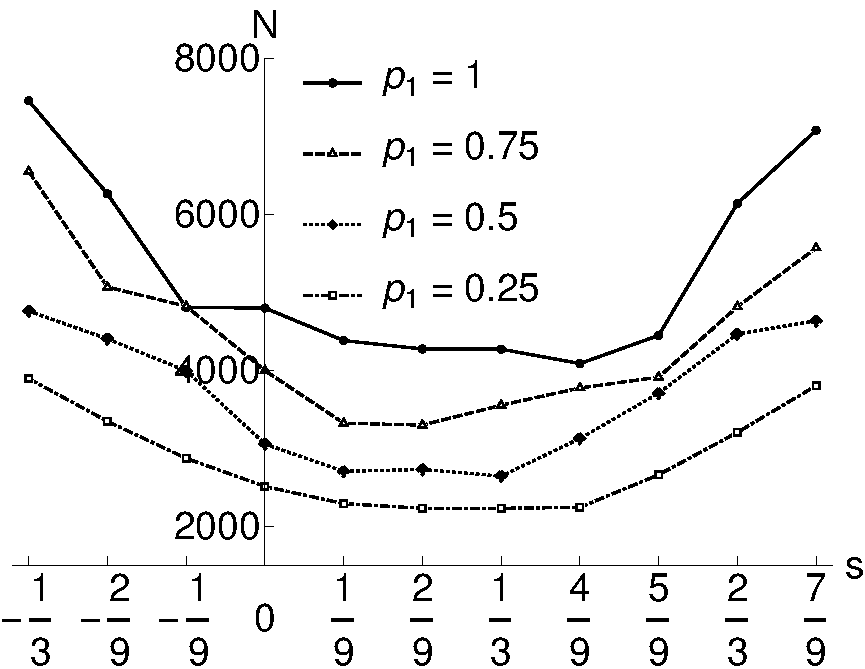
\includegraphics[width=\linewidth]{pics/MechanicalIter.pdf} \\ б)
    \end{minipage}
    \caption{Зависимость (а) числа обусловленности и (б) количества итераций $N$ для матрицы жёсткости $\widehat{\textbf{K}}_E$ от параметров $s$ и $p_1$ при $r = 0.1$}
    \label{fig:MechanicalCondAndIter}
\end{figure}

\section{Предобуславливание и выбор начального приближения}\label{sec:NumericalMethods/Preconditioning}

Оптимизированный базис квадратичных серендиповых элементов позволил ускорить сходимость метода сопряжённых градиентов при решении СЛАУ более чем в 1.5 раза по сравнению со случаем, когда используется классический базис. Однако существует возможность добиться ещё большей скорости сходимости за счёт использования предобуславливателей или более подходящих начальных условий.

При разработке предобуславливателя важно учитывать специфику задачи, так как универсальных способов эффективного предобуславливания не существует. Также важно учитывать возможности современных вычислительных машин: параллельные вычисления зачастую дают заметно больший выигрыш во времени, в отличие от предобуславливания в силу того, что многие популярные методы предобуславливания используют обратный алгоритм Гаусса, который не всегда возможно эффективно распараллелить, а накладные расходы при этом могут значительно увеличить цену одной итерации.

Пожалуй основной спецификой рассматриваемого класса уравнений является их матрично-векторное представление (\ref{eq:ThermalSLAE}) и (\ref{eq:StressSLAE}), где матричные выражения представлены в виде взвешенных сумм локальных $\widehat{\textbf{K}}^L_{\mathcal{F}}$ и нелокальных $\widehat{\textbf{K}}^{NL}_{\mathcal{F}}$ матриц. При этом локальные слагаемые обалают заметно меньшей плотностью заполнения, чем нелокальные. Учитывая эту специфику, а также уже рассмотренный анализ границ спектров матриц $\widehat{\textbf{K}}_{\mathcal{F}}$, можем построить предобуславливатель используя для этого лишь локальное слагаемое.

Как правило для построения предобуславливателей необходимы данные о максимальных и минимальных собственных числах, однако, процесс нахождения границ спектра, даже для локальной матрицы, является слишком медленным. Поэтому примем во внимание полученные знания о связи спектров локальной и полной матриц и в качестве предобуславливателя возьмём неполное разложение Холецкого локальной матрицы $\widehat{\textbf{K}}^L_{\mathcal{F}}$, так как оно не требует непосредственного поиска собственных чисел.

Теперь проведём серию расчётов и на её основе определим эффективность использования предобуславливателя. В этом же исследовании проверим гипотезу о выборе начального приближения, где в качестве начального приближения выберем результат решения СЛАУ $\widehat{\textbf{K}}^L_{\mathcal{F}} \cdot \textbf{X}_0 = \textbf{F}$, где $\textbf{F}$ --- вектор правой части, на основе которого будем решать полную СЛАУ и $\textbf{X}_0$ --- вектор искомого начального приближения. Для теста будем рассматривать задачи из предыдущего раздела, а базис элементов выберем оптимальным с параметром $s = 2/9$.

По результатам, представленным в Таблицах \ref{tab:ThermalPrecond} и \ref{tab:StressPrecond} для уравнений теплопроводности и равновесия соотвественно, можем сделать вывод, что использование предобуславливателя позволяет ускорить решение СЛАУ в N раз. При этом весовые параметры модели на это не оказывают серьёзного влияния. Вместе с этим можно сделать вывод касательно выбора начального приближения. Однако предложенная гипотеза не даёт ожидаемого эффекта, количество итераций сокращается несущественно, а время затрачиваемое на решение СЛАУ для классической задачи не всегда меньше получаемого выигрыша. В качестве замечания стоит добавить, что для краткости записи формулировка в таблице ILLT$\left( \widehat{\textbf{K}}^L_T \right)$ означает использование предобуславливателя, а ILLT$\left( \widehat{\textbf{K}}^L_T \right) + X_0$ подразумевает комбинацию предобуславливания и начального приближения.

\begin{table}[htbp]
    \centering
    \begin{threeparttable}% выравнивание подписи по границам таблицы
        \caption{Количество итераций и затрачиваемое время при решении СЛАУ уравнения теплопроводности}\label{tab:ThermalPrecond}
        \begin{tabular}{|c|c|c|c|c|c|c|}
		\hline
		$p_1$ & \multicolumn{2}{c|}{Без предобуславливания} & \multicolumn{2}{c|}{ILLT$\left( \widehat{\textbf{K}}^L_T \right)$} & \multicolumn{2}{c|}{ILLT$\left( \widehat{\textbf{K}}^L_T \right) + X_0$}\\
		\cline{2-7}
		     & $N$ & $t$, с & $N$ & $t$, с & $N$ & $t$, с \\
		\hline
		0.75 & 5364 & 2970 & 2111 & 1181 & 2086 & 1238 (1167) \\
		\hline
		0.5  & 4558 & 2527 & 1740 & 972 & 1742 & 1045 (974) \\
		\hline
		0.25 & 3020 & 1673 & 1250 & 657 & 1265 & 779 (708) \\
		\hline
        \end{tabular}
    \end{threeparttable}
\end{table}

\begin{table}[htbp]
    \centering
    \begin{threeparttable}% выравнивание подписи по границам таблицы
        \caption{Количество итераций и затрачиваемое время при решении СЛАУ уравнения равновесия}\label{tab:StressPrecond}
        \begin{tabular}{|c|c|c|c|c|c|c|}
		\hline
		$p_1$ & \multicolumn{2}{c|}{Без предобуславливания} & \multicolumn{2}{c|}{ILLT$\left( \widehat{\textbf{K}}^L_T \right)$} & \multicolumn{2}{c|}{ILLT$\left( \widehat{\textbf{K}}^L_T \right) + X_0$}\\
		\cline{2-7}
		     & $N$ & $t$, с & $N$ & $t$, с & $N$ & $t$, с \\
		\hline
		0.75 & 6330 & 13238 & 2902 & 6217 & 2736 & 6223 (5967) \\
		\hline
		0.5  & 5167 & 10811 & 2290 & 4915 & 2389 & 5442 (5203) \\
		\hline
		0.25 & 3779 & 7888 & 1718 & 3695 & 1740 & 4032 (3793) \\
		\hline
        \end{tabular}
    \end{threeparttable}
\end{table}

\section{Основные результаты и выводы по главе 5}\label{sec:NonLocFEMAnalysis/Conclusion}

\begin{enumerate}
	\item Исследована масштабируемость программного комплекса NonLocFEM на машинах с общей и распределённой памятью. Представленные результаты демонстрируют хорошую эффективность распараллеливания, выполненную средствами OpenMP, и балансировку данных между процессами, при использовании технологии MPI.
	
	\item Проведён анализ скорости сходимости метода споряжённых градиентов при вариации базиса квадратичного серендипового элемента. Показано, что оценка, предложенная в разделе \ref{sec:ProgramComplex/BasisOptimization}, даёт корректный результат и минимум числа обусловленности матриц теплопроводности и жёсткости, а также наибольшая скорость сходимости метода сопряжённых градиентов, находятся в окрестности точки $s = 2/9$.
	
	\item Предложенный способ предобуславливания на основе неполного разложения Холецкого локальных матриц, продемонстрировал существенный прирост в скорости сходимости метода сопряжённых градиентов, при решении уравнений теплопроводности и равновесия в нелокальных постановках.
\end{enumerate}